\chapter{Differentiation: Instantaneous Rate of Change}

\section{From Continuity to Differentiability}

\begin{intuition}
Continuity asks: ``Does the function have jumps?''

Differentiability asks: ``Does the function have sharp corners?''

\textbf{The derivative} $f'(x)$ measures the \textbf{instantaneous rate of change} of $f$ at $x$:
\begin{itemize}
    \item Geometrically: Slope of the tangent line
    \item Physically: Velocity (if $f$ is position)
    \item Economically: Marginal cost/revenue
\end{itemize}

This chapter develops differentiation rigorously from limits.
\end{intuition}

\begin{historicalnote}
\textbf{The Birth of Calculus}

\textbf{Ancient Precursors (c. 250 BCE - 1600 CE)}:
\begin{itemize}
    \item \textbf{Archimedes}: Computed tangent lines to spirals (geometric methods)
    \item \textbf{Fermat (1629)}: Method of ``adequality'' (proto-derivatives)
    \item \textbf{Barrow (1670)}: Geometric tangent method (Newton's teacher)
\end{itemize}

\textbf{The Revolution (1665-1675)}:
\begin{itemize}
    \item \textbf{Newton (1665)}: ``Fluxions''---rates of change of ``fluents''
    \item \textbf{Leibniz (1675)}: Notation $\frac{dy}{dx}$, infinitesimals $dx$, $dy$
    \item Both discovered: Differentiation and integration are inverse operations
    \item \textbf{Priority dispute}: One of history's most bitter mathematical feuds
\end{itemize}

\textbf{The Rigor Gap (1700-1850)}:
\begin{itemize}
    \item Euler, Lagrange, Laplace: Manipulated derivatives powerfully but non-rigorously
    \item \textbf{Berkeley's attack (1734)}: ``What are these infinitesimals? Ghosts of departed quantities!''
    \item No answer: Infinitesimals weren't properly defined
\end{itemize}

\textbf{19th Century Foundations}:
\begin{itemize}
    \item \textbf{Cauchy (1821)}: First limit-based definition of derivative
    \item \textbf{Weierstrass (1860s)}: Rigorous $\epsilon$-$\delta$ formulation
    \item \textbf{Dedekind (1872)}: Completed $\mathbb{R}$, making all limits rigorous
    \item Result: Calculus became a branch of analysis with complete proofs
\end{itemize}

\textbf{Modern View}: Derivatives are limits. Infinitesimals can be made rigorous (non-standard analysis, 1960s) but are not needed for standard calculus.
\end{historicalnote}

\section{The Derivative: Definition and Interpretation}

\begin{definition}[Derivative at a Point]
Let $f: D \to \mathbb{R}$ where $D \subseteq \mathbb{R}$, and let $c \in D$ be an interior point (not an endpoint).

The \textbf{derivative of $f$ at $c$} is:
\[f'(c) = \lim_{h \to 0} \frac{f(c + h) - f(c)}{h}\]

provided this limit exists.

If the limit exists, we say $f$ is \textbf{differentiable at $c$}.

\textbf{Alternative form} (using $x$ instead of $c + h$):
\[f'(c) = \lim_{x \to c} \frac{f(x) - f(c)}{x - c}\]
\end{definition}

\begin{keyidea}
\textbf{The difference quotient} $\frac{f(c+h) - f(c)}{h}$ is the \textbf{average rate of change} of $f$ over the interval $[c, c+h]$.

As $h \to 0$, this becomes the \textbf{instantaneous rate of change}.

\textbf{Geometric interpretation}:
\begin{center}
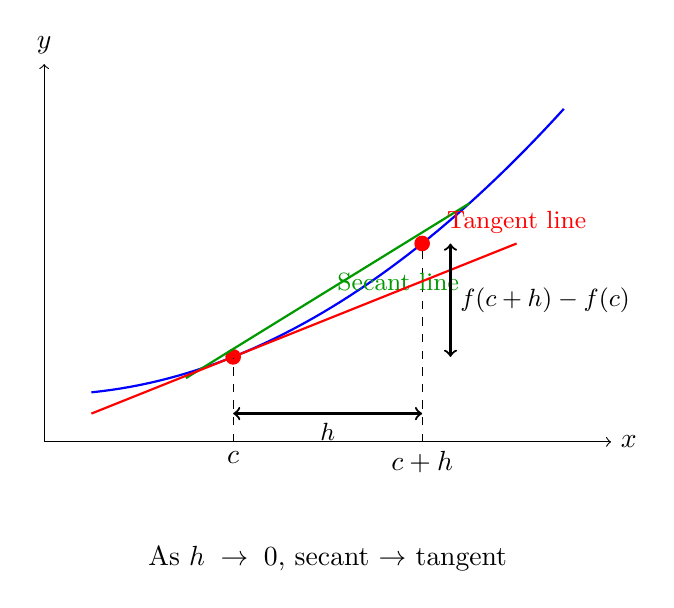
\begin{tikzpicture}[scale=1.2]
    \draw[->] (0, 0) -- (6, 0) node[right] {$x$};
    \draw[->] (0, 0) -- (0, 4) node[above] {$y$};
    
    % Function curve
    \draw[thick, blue, domain=0.5:5.5, samples=50] plot (\x, {0.1*\x*\x + 0.5});
    
    % Point c
    \node[circle, fill=red, inner sep=2pt] (c) at (2, 0.9) {};
    \node[below] at (2, 0) {$c$};
    \draw[dashed] (2, 0) -- (2, 0.9);
    
    % Point c+h
    \node[circle, fill=red, inner sep=2pt] (ch) at (4, 2.1) {};
    \node[below] at (4, 0) {$c+h$};
    \draw[dashed] (4, 0) -- (4, 2.1);
    
    % Secant line
    \draw[thick, green!60!black] (1.5, 0.675) -- (4.5, 2.525);
    \node[above right, font=\small] at (3, 1.5) {\textcolor{green!60!black}{Secant line}};
    
    % Tangent line
    \draw[thick, red, domain=0.5:5, samples=50] plot (\x, {0.4*\x + 0.1});
    \node[above, font=\small] at (5, 2.1) {\textcolor{red}{Tangent line}};
    
    % Differences
    \draw[<->, thick] (4, 0.3) -- (2, 0.3);
    \node[below, font=\small] at (3, 0.3) {$h$};
    
    \draw[<->, thick] (4.3, 0.9) -- (4.3, 2.1);
    \node[right, font=\small] at (4.3, 1.5) {$f(c+h) - f(c)$};
    
    \node[below, text width=6cm, align=center] at (3, -1) {
        As $h \to 0$, secant $\to$ tangent
    };
\end{tikzpicture}
\end{center}

The derivative $f'(c)$ is the slope of the tangent line at $x = c$.
\end{keyidea}

\begin{example}[Computing a Derivative from Definition]
Find the derivative of $f(x) = x^2$ at $c = 3$.

\textbf{Solution}:
\begin{align*}
f'(3) &= \lim_{h \to 0} \frac{f(3 + h) - f(3)}{h} \\
&= \lim_{h \to 0} \frac{(3 + h)^2 - 9}{h} \\
&= \lim_{h \to 0} \frac{9 + 6h + h^2 - 9}{h} \\
&= \lim_{h \to 0} \frac{6h + h^2}{h} \\
&= \lim_{h \to 0} \frac{h(6 + h)}{h} \\
&= \lim_{h \to 0} (6 + h) \\
&= 6
\end{align*}

Therefore $f'(3) = 6$. $\blacksquare$

(More generally, for $f(x) = x^2$, we get $f'(c) = 2c$ for any $c$.)
\end{example}

\begin{example}[Function Not Differentiable]
Consider $f(x) = |x|$ at $c = 0$.

\textbf{Right-hand derivative}:
\[\lim_{h \to 0^+} \frac{|h| - 0}{h} = \lim_{h \to 0^+} \frac{h}{h} = 1\]

\textbf{Left-hand derivative}:
\[\lim_{h \to 0^-} \frac{|h| - 0}{h} = \lim_{h \to 0^-} \frac{-h}{h} = -1\]

Since the left and right limits disagree, $\lim_{h \to 0} \frac{|h|}{h}$ does not exist.

Therefore $f(x) = |x|$ is not differentiable at $x = 0$ (sharp corner). $\blacksquare$
\end{example}

\begin{definition}[Derivative Function]
If $f$ is differentiable at every point in its domain, the \textbf{derivative function} is:
\[f': D \to \mathbb{R}, \quad f'(x) = \lim_{h \to 0} \frac{f(x + h) - f(x)}{h}\]

\textbf{Notations}:
\[f'(x) = \frac{df}{dx} = \frac{d}{dx}f(x) = Df(x) = D_x f\]
\end{definition}

\section{Differentiability Implies Continuity}

\begin{theorem}
If $f$ is differentiable at $c$, then $f$ is continuous at $c$.
\end{theorem}

\begin{proof}
Assume $f$ is differentiable at $c$, so $f'(c) = \lim_{h \to 0} \frac{f(c+h) - f(c)}{h}$ exists.

We need to show $\lim_{h \to 0} f(c + h) = f(c)$, i.e., $\lim_{h \to 0} [f(c+h) - f(c)] = 0$.

Note that:
\[f(c + h) - f(c) = \frac{f(c+h) - f(c)}{h} \cdot h\]

Taking limits as $h \to 0$:
\begin{align*}
\lim_{h \to 0} [f(c+h) - f(c)] &= \lim_{h \to 0} \left[\frac{f(c+h) - f(c)}{h} \cdot h\right] \\
&= \left[\lim_{h \to 0} \frac{f(c+h) - f(c)}{h}\right] \cdot \left[\lim_{h \to 0} h\right] \\
&= f'(c) \cdot 0 = 0
\end{align*}

Therefore $f(c + h) \to f(c)$ as $h \to 0$, so $f$ is continuous at $c$. $\blacksquare$
\end{proof}

\begin{warning}
The converse is \textbf{false}: Continuity does not imply differentiability.

\textbf{Example}: $f(x) = |x|$ is continuous at $0$ but not differentiable at $0$.

\textbf{More extreme}: Weierstrass (1872) constructed a function continuous \textit{everywhere} but differentiable \textit{nowhere}---a continuous but infinitely jagged curve!
\end{warning}

\begin{center}
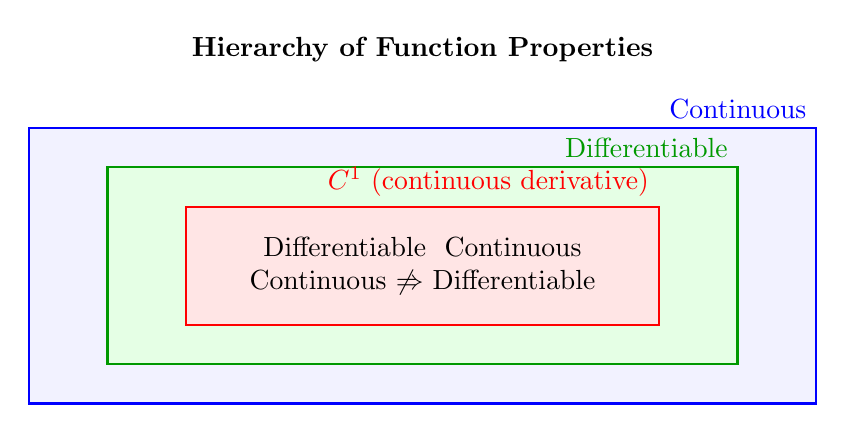
\begin{tikzpicture}[scale=1.0]
    \node at (6, 5) {\textbf{Hierarchy of Function Properties}};
    
    % Nested boxes
    \draw[thick, blue, fill=blue!5] (1, 0.5) rectangle (11, 4);
    \node[above left] at (11, 4) {\textcolor{blue}{Continuous}};
    
    \draw[thick, green!60!black, fill=green!10] (2, 1) rectangle (10, 3.5);
    \node[above left] at (10, 3.5) {\textcolor{green!60!black}{Differentiable}};
    
    \draw[thick, red, fill=red!10] (3, 1.5) rectangle (9, 3);
    \node[above left] at (9, 3) {\textcolor{red}{$C^1$ (continuous derivative)}};
    
    \node[text width=5cm, align=center] at (6, 2.25) {
        Differentiable $\implies$ Continuous \\
        Continuous $\not\Rightarrow$ Differentiable
    };
\end{tikzpicture}
\end{center}

\section{Differentiation Rules}

\begin{theorem}[Power Rule]
For $f(x) = x^n$ where $n \in \mathbb{N}$:
\[f'(x) = nx^{n-1}\]
\end{theorem}

\begin{proof}
We use the binomial theorem:
\begin{align*}
f'(c) &= \lim_{h \to 0} \frac{(c + h)^n - c^n}{h} \\
&= \lim_{h \to 0} \frac{1}{h}\left[\sum_{k=0}^n \binom{n}{k} c^{n-k} h^k - c^n\right] \\
&= \lim_{h \to 0} \frac{1}{h}\left[c^n + nc^{n-1}h + \binom{n}{2}c^{n-2}h^2 + \cdots + h^n - c^n\right] \\
&= \lim_{h \to 0} \left[nc^{n-1} + \binom{n}{2}c^{n-2}h + \cdots + h^{n-1}\right] \\
&= nc^{n-1}
\end{align*}

Therefore $(x^n)' = nx^{n-1}$. $\blacksquare$
\end{proof}

\begin{theorem}[Algebra of Derivatives]
If $f$ and $g$ are differentiable at $c$, then:
\begin{enumerate}
    \item \textbf{Constant multiple}: $(cf)' = cf'$ for any $c \in \mathbb{R}$
    \item \textbf{Sum rule}: $(f + g)' = f' + g'$
    \item \textbf{Product rule}\index{product rule}\index{differentiation!product rule}: $(fg)' = f'g + fg'$
    \item \textbf{Quotient rule}\index{quotient rule}\index{differentiation!quotient rule}: $\left(\frac{f}{g}\right)' = \frac{f'g - fg'}{g^2}$ (if $g(c) \neq 0$)
\end{enumerate}
\end{theorem}

\begin{proof}[Proof of Product Rule]
\begin{align*}
(fg)'(c) &= \lim_{h \to 0} \frac{f(c+h)g(c+h) - f(c)g(c)}{h}
\end{align*}

\textbf{Trick}: Add and subtract $f(c+h)g(c)$:
\begin{align*}
&= \lim_{h \to 0} \frac{f(c+h)g(c+h) - f(c+h)g(c) + f(c+h)g(c) - f(c)g(c)}{h} \\
&= \lim_{h \to 0} \left[f(c+h) \cdot \frac{g(c+h) - g(c)}{h} + g(c) \cdot \frac{f(c+h) - f(c)}{h}\right] \\
&= \lim_{h \to 0} f(c+h) \cdot \lim_{h \to 0} \frac{g(c+h) - g(c)}{h} + g(c) \cdot \lim_{h \to 0} \frac{f(c+h) - f(c)}{h} \\
&= f(c) \cdot g'(c) + g(c) \cdot f'(c) \quad \text{(using continuity of $f$)}
\end{align*}

Therefore $(fg)' = f'g + fg'$. $\blacksquare$
\end{proof}

\begin{proof}[Proof of Quotient Rule]
Let $h(x) = \frac{f(x)}{g(x)}$ where $g(c) \neq 0$.

\begin{align*}
h'(c) &= \lim_{x \to c} \frac{h(x) - h(c)}{x - c} \\
&= \lim_{x \to c} \frac{\frac{f(x)}{g(x)} - \frac{f(c)}{g(c)}}{x - c} \\
&= \lim_{x \to c} \frac{f(x)g(c) - f(c)g(x)}{(x - c)g(x)g(c)}
\end{align*}

\textbf{Trick}: Add and subtract $f(c)g(c)$ in the numerator:
\begin{align*}
&= \lim_{x \to c} \frac{f(x)g(c) - f(c)g(c) + f(c)g(c) - f(c)g(x)}{(x - c)g(x)g(c)} \\
&= \lim_{x \to c} \frac{[f(x) - f(c)]g(c) - f(c)[g(x) - g(c)]}{(x - c)g(x)g(c)} \\
&= \lim_{x \to c} \left[\frac{f(x) - f(c)}{x - c} \cdot \frac{g(c)}{g(x)g(c)} - \frac{f(c)}{g(c)} \cdot \frac{g(x) - g(c)}{x - c} \cdot \frac{1}{g(x)}\right] \\
&= f'(c) \cdot \frac{1}{g(c)} - \frac{f(c)}{g(c)} \cdot g'(c) \cdot \frac{1}{g(c)} \\
&= \frac{f'(c)g(c) - f(c)g'(c)}{g(c)^2}
\end{align*}

Therefore $\left(\frac{f}{g}\right)' = \frac{f'g - fg'}{g^2}$. $\blacksquare$
\end{proof}

\begin{example}[Using Differentiation Rules]
Find the derivative of $h(x) = (3x^2 + 5x)(x^3 - 2)$.

\textbf{Method 1 (Product rule)}:
\begin{align*}
h'(x) &= (3x^2 + 5x)' \cdot (x^3 - 2) + (3x^2 + 5x) \cdot (x^3 - 2)' \\
&= (6x + 5)(x^3 - 2) + (3x^2 + 5x)(3x^2) \\
&= 6x^4 - 12x + 5x^3 - 10 + 9x^4 + 15x^3 \\
&= 15x^4 + 20x^3 - 12x - 10
\end{align*}

\textbf{Method 2 (Expand first)}:
\[h(x) = 3x^5 + 5x^4 - 6x^2 - 10x\]
\[h'(x) = 15x^4 + 20x^3 - 12x - 10\]

Both methods agree. $\checkmark$
\end{example}

\begin{theorem}[Chain Rule]\index{chain rule}\index{differentiation!chain rule}
If $g$ is differentiable at $c$ and $f$ is differentiable at $g(c)$, then $f \circ g$ is differentiable at $c$, and:
\[(f \circ g)'(c) = f'(g(c)) \cdot g'(c)\]

In Leibniz notation: If $y = f(u)$ and $u = g(x)$, then:
\[\frac{dy}{dx} = \frac{dy}{du} \cdot \frac{du}{dx}\]
\end{theorem}

\begin{proof}[Proof Sketch]
The intuitive ``proof'' is:
\[\frac{dy}{dx} = \frac{dy}{du} \cdot \frac{du}{dx}\]
(``canceling'' $du$).

But $\frac{dy}{dx}$ is not a fraction---it's a limit! The rigorous proof is more subtle.

Define $\phi(h) = \frac{g(c+h) - g(c)}{h} - g'(c)$ for $h \neq 0$, and $\phi(0) = 0$.

Then $\phi(h) \to 0$ as $h \to 0$ (by definition of $g'(c)$), and:
\[g(c + h) = g(c) + [g'(c) + \phi(h)]h\]

Let $k = g(c + h) - g(c)$. Similarly:
\[f(g(c) + k) = f(g(c)) + [f'(g(c)) + \psi(k)]k\]

where $\psi(k) \to 0$ as $k \to 0$.

Substituting:
\begin{align*}
(f \circ g)(c + h) &= f(g(c + h)) \\
&= f(g(c) + k) \\
&= f(g(c)) + [f'(g(c)) + \psi(k)]k \\
&= f(g(c)) + [f'(g(c)) + \psi(k)][g'(c) + \phi(h)]h
\end{align*}

Therefore:
\[\frac{(f \circ g)(c+h) - (f \circ g)(c)}{h} = [f'(g(c)) + \psi(k)][g'(c) + \phi(h)]\]

Taking $h \to 0$ (which forces $k \to 0$ by continuity of $g$):
\[(f \circ g)'(c) = f'(g(c)) \cdot g'(c)\]
$\blacksquare$
\end{proof}

\begin{example}[Chain Rule]
Find the derivative of $h(x) = (x^2 + 3x)^5$.

\textbf{Solution}: Let $f(u) = u^5$ and $g(x) = x^2 + 3x$. Then $h = f \circ g$.

By chain rule:
\begin{align*}
h'(x) &= f'(g(x)) \cdot g'(x) \\
&= 5(g(x))^4 \cdot (2x + 3) \\
&= 5(x^2 + 3x)^4 \cdot (2x + 3)
\end{align*}
$\blacksquare$
\end{example}

\section{The Mean Value Theorem}

\begin{intuition}
If you drive 100 miles in 2 hours, at some moment your instantaneous speed was exactly 50 mph (the average).

More generally: Between any two points on a differentiable curve, there's a point where the tangent line is parallel to the secant line.

This simple-sounding theorem has profound consequences for all of analysis.
\end{intuition}

\begin{theorem}[Rolle's Theorem]\index{Rolle's theorem}\index{mean value theorem!Rolle's theorem}
Let $f: [a, b] \to \mathbb{R}$ be continuous on $[a, b]$ and differentiable on $(a, b)$.

If $f(a) = f(b)$, then there exists $c \in (a, b)$ such that $f'(c) = 0$.
\end{theorem}

\begin{center}
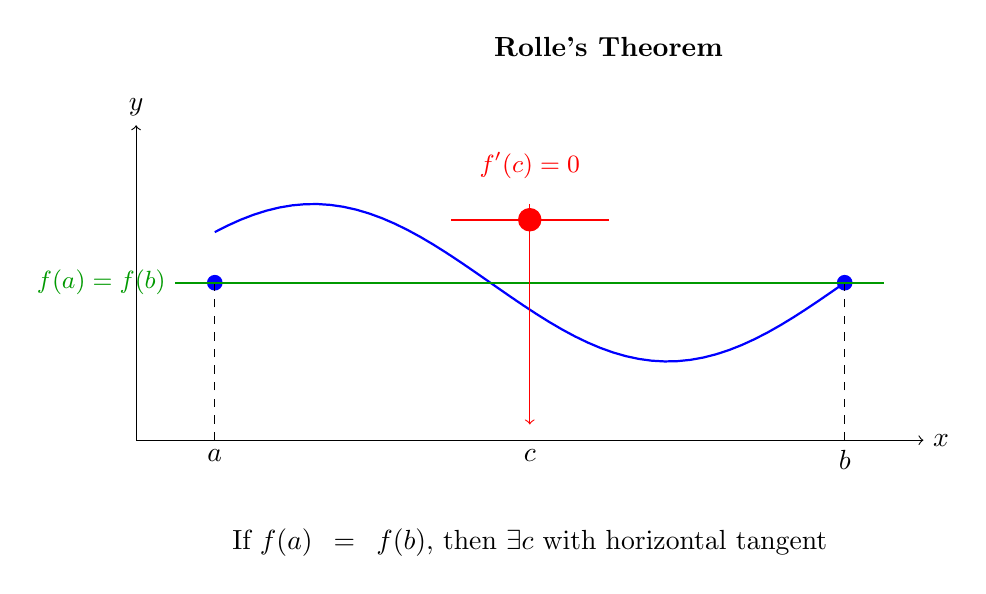
\begin{tikzpicture}[scale=1.0]
    \node at (6, 5) {\textbf{Rolle's Theorem}};
    
    \draw[->] (0, 0) -- (10, 0) node[right] {$x$};
    \draw[->] (0, 0) -- (0, 4) node[above] {$y$};
    
    % Function curve (starts and ends at same height)
    \draw[thick, blue, domain=1:9, samples=50] plot (\x, {2 + sin(40*\x)});
    
    % Points a and b
    \node[circle, fill=blue, inner sep=2pt] at (1, 2) {};
    \node[below] at (1, 0) {$a$};
    \draw[dashed] (1, 0) -- (1, 2);
    
    \node[circle, fill=blue, inner sep=2pt] at (9, 2) {};
    \node[below] at (9, 0) {$b$};
    \draw[dashed] (9, 0) -- (9, 2);
    
    % Horizontal secant line
    \draw[thick, green!60!black] (0.5, 2) -- (9.5, 2);
    \node[left, font=\small] at (0.5, 2) {\textcolor{green!60!black}{$f(a) = f(b)$}};
    
    % Point c where f'(c) = 0
    \node[circle, fill=red, inner sep=3pt] at (5, 2.8) {};
    \draw[thick, red] (4, 2.8) -- (6, 2.8);
    \node[above, font=\small] at (5, 3.2) {\textcolor{red}{$f'(c) = 0$}};
    \draw[->, red] (5, 3) -- (5, 0.2);
    \node[below] at (5, 0) {$c$};
    
    \node[below, text width=10cm, align=center] at (5, -1) {
        If $f(a) = f(b)$, then $\exists c$ with horizontal tangent
    };
\end{tikzpicture}
\end{center}

\begin{proof}
Since $f$ is continuous on $[a, b]$, by EVT, $f$ attains its maximum and minimum.

\textbf{Case 1}: If $f$ is constant, then $f'(x) = 0$ for all $x \in (a, b)$. Done. $\checkmark$

\textbf{Case 2}: If $f$ is not constant, then either the maximum or minimum occurs at an interior point $c \in (a, b)$ (since $f(a) = f(b)$, they can't both be at endpoints if $f$ is non-constant).

Without loss of generality, assume $f$ attains its maximum at $c \in (a, b)$.

Then $f(c) \geq f(x)$ for all $x \in [a, b]$.

For $h > 0$ small:
\[\frac{f(c + h) - f(c)}{h} \leq 0 \quad \text{(since $f(c + h) \leq f(c)$)}\]

Taking $h \to 0^+$: $f'(c) \leq 0$.

For $h < 0$ small:
\[\frac{f(c + h) - f(c)}{h} \geq 0 \quad \text{(negative divided by negative)}\]

Taking $h \to 0^-$: $f'(c) \geq 0$.

Therefore $f'(c) = 0$. $\blacksquare$
\end{proof}

\begin{theorem}[Mean Value Theorem (MVT)]\index{mean value theorem}\index{MVT}\index{differentiation!mean value theorem}
Let $f: [a, b] \to \mathbb{R}$ be continuous on $[a, b]$ and differentiable on $(a, b)$.

Then there exists $c \in (a, b)$ such that:
\[f'(c) = \frac{f(b) - f(a)}{b - a}\]

\textbf{In words}: The instantaneous rate of change at some point equals the average rate of change.
\end{theorem}

\begin{center}
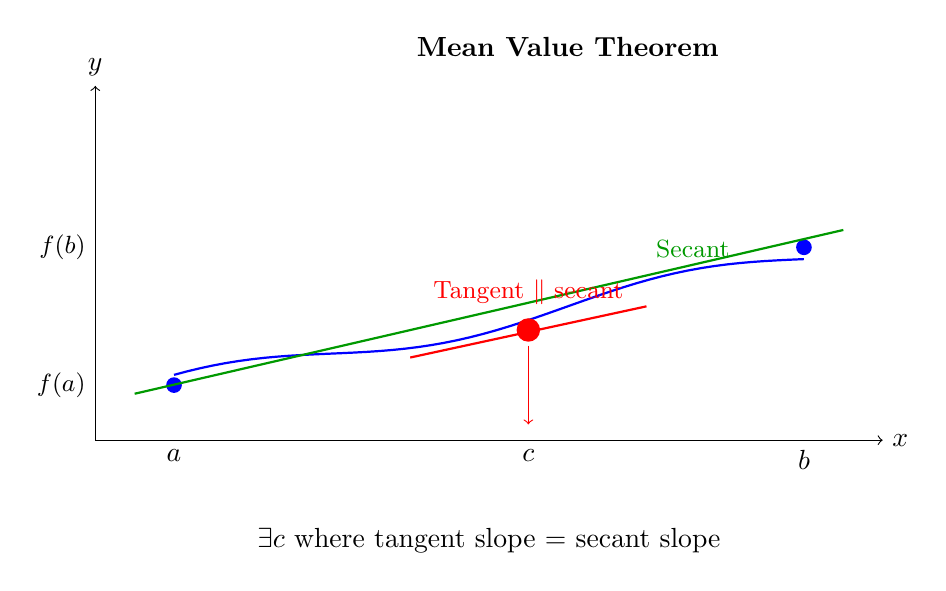
\begin{tikzpicture}[scale=1.0]
    \node at (6, 5) {\textbf{Mean Value Theorem}};
    
    \draw[->] (0, 0) -- (10, 0) node[right] {$x$};
    \draw[->] (0, 0) -- (0, 4.5) node[above] {$y$};
    
    % Function curve
    \draw[thick, blue, domain=1:9, samples=50] plot (\x, {0.5 + 0.2*\x + 0.15*sin(60*\x)});
    
    % Points a and b
    \node[circle, fill=blue, inner sep=2pt] at (1, 0.7) {};
    \node[below] at (1, 0) {$a$};
    \node[left, font=\small] at (0, 0.7) {$f(a)$};
    
    \node[circle, fill=blue, inner sep=2pt] at (9, 2.45) {};
    \node[below] at (9, 0) {$b$};
    \node[left, font=\small] at (0, 2.45) {$f(b)$};
    
    % Secant line
    \draw[thick, green!60!black] (0.5, 0.59) -- (9.5, 2.67);
    \node[above right, font=\small] at (7, 2.2) {\textcolor{green!60!black}{Secant}};
    
    % Tangent line parallel to secant
    \draw[thick, red] (4, 1.05) -- (7, 1.7);
    \node[above, font=\small] at (5.5, 1.6) {\textcolor{red}{Tangent $\parallel$ secant}};
    
    % Point c
    \node[circle, fill=red, inner sep=3pt] at (5.5, 1.4) {};
    \draw[->, red] (5.5, 1.2) -- (5.5, 0.2);
    \node[below] at (5.5, 0) {$c$};
    
    \node[below, text width=10cm, align=center] at (5, -1) {
        $\exists c$ where tangent slope $=$ secant slope
    };
\end{tikzpicture}
\end{center}

\begin{proof}
Define an auxiliary function that measures the vertical distance from the secant line:
\[g(x) = f(x) - \left[f(a) + \frac{f(b) - f(a)}{b - a}(x - a)\right]\]

(The term in brackets is the secant line through $(a, f(a))$ and $(b, f(b))$.)

\textbf{Properties of $g$}:
\begin{itemize}
    \item $g$ is continuous on $[a, b]$ and differentiable on $(a, b)$ (since $f$ is)
    \item $g(a) = f(a) - f(a) = 0$
    \item $g(b) = f(b) - f(b) = 0$
\end{itemize}

By Rolle's Theorem, there exists $c \in (a, b)$ with $g'(c) = 0$.

But:
\[g'(x) = f'(x) - \frac{f(b) - f(a)}{b - a}\]

Therefore:
\[0 = g'(c) = f'(c) - \frac{f(b) - f(a)}{b - a}\]

Rearranging:
\[f'(c) = \frac{f(b) - f(a)}{b - a}\]
$\blacksquare$
\end{proof}

\begin{keyidea}
\textbf{MVT is the foundation of differential calculus}. Almost every major theorem follows from it:
\begin{itemize}
    \item $f' = 0 \implies f$ is constant
    \item $f' > 0 \implies f$ is increasing
    \item $f' = g' \implies f = g + C$
    \item Taylor's theorem (approximating functions by polynomials)
\end{itemize}
\end{keyidea}

\section{Consequences of the Mean Value Theorem}

\begin{theorem}[Zero Derivative Implies Constant]
If $f'(x) = 0$ for all $x \in (a, b)$, then $f$ is constant on $(a, b)$.
\end{theorem}

\begin{proof}
Let $x_1, x_2 \in (a, b)$ with $x_1 < x_2$.

By MVT applied to $[x_1, x_2]$, there exists $c \in (x_1, x_2)$ such that:
\[f(x_2) - f(x_1) = f'(c)(x_2 - x_1)\]

Since $f'(c) = 0$:
\[f(x_2) - f(x_1) = 0 \implies f(x_2) = f(x_1)\]

Since $x_1, x_2$ were arbitrary, $f$ is constant. $\blacksquare$
\end{proof}

\begin{theorem}[Increasing/Decreasing Test]
Let $f$ be continuous on $[a, b]$ and differentiable on $(a, b)$.
\begin{enumerate}
    \item If $f'(x) > 0$ for all $x \in (a, b)$, then $f$ is strictly increasing on $[a, b]$
    \item If $f'(x) < 0$ for all $x \in (a, b)$, then $f$ is strictly decreasing on $[a, b]$
    \item If $f'(x) \geq 0$ for all $x \in (a, b)$, then $f$ is increasing on $[a, b]$
\end{enumerate}
\end{theorem}

\begin{proof}[Proof of (1)]
Let $x_1 < x_2$ in $[a, b]$.

By MVT, there exists $c \in (x_1, x_2)$ such that:
\[f(x_2) - f(x_1) = f'(c)(x_2 - x_1)\]

Since $f'(c) > 0$ and $x_2 - x_1 > 0$:
\[f(x_2) - f(x_1) > 0 \implies f(x_2) > f(x_1)\]

Therefore $f$ is strictly increasing. $\blacksquare$
\end{proof}

\begin{example}[Finding Intervals of Increase/Decrease]
Let $f(x) = x^3 - 3x^2 + 2$. Find where $f$ is increasing and decreasing.

\textbf{Solution}:
\[f'(x) = 3x^2 - 6x = 3x(x - 2)\]

\textbf{Critical points}: $f'(x) = 0$ when $x = 0$ or $x = 2$.

\textbf{Sign analysis}:
\begin{itemize}
    \item $x < 0$: $f'(x) = 3(-)(-) = (+) > 0$ $\implies$ $f$ increasing
    \item $0 < x < 2$: $f'(x) = 3(+)(-) = (-) < 0$ $\implies$ $f$ decreasing
    \item $x > 2$: $f'(x) = 3(+)(+) = (+) > 0$ $\implies$ $f$ increasing
\end{itemize}

Therefore: $f$ increases on $(-\infty, 0]$, decreases on $[0, 2]$, increases on $[2, \infty)$. $\blacksquare$
\end{example}

\begin{theorem}[Antiderivatives Differ by a Constant]
If $f'(x) = g'(x)$ for all $x \in (a, b)$, then there exists a constant $C$ such that $f(x) = g(x) + C$ for all $x \in (a, b)$.
\end{theorem}

\begin{proof}
Let $h(x) = f(x) - g(x)$.

Then $h'(x) = f'(x) - g'(x) = 0$ for all $x \in (a, b)$.

By the previous theorem, $h$ is constant, say $h(x) = C$.

Therefore $f(x) - g(x) = C$, i.e., $f(x) = g(x) + C$. $\blacksquare$
\end{proof}

\begin{keyidea}
This theorem justifies the ``$+C$'' in antiderivatives:

If $F'(x) = f(x)$, then \textit{any} antiderivative of $f$ has the form $F(x) + C$.

This is why indefinite integrals always include $+C$!
\end{keyidea}

\section{Higher Derivatives and Concavity}

\begin{definition}[Higher Derivatives]
If $f'$ is differentiable, we define the \textbf{second derivative}:
\[f''(x) = (f')'(x) = \frac{d^2f}{dx^2}\]

Similarly: $f'''$ (third derivative), $f^{(4)}$ (fourth), ..., $f^{(n)}$ ($n$-th derivative).

A function is \textbf{$C^n$} if $f^{(n)}$ exists and is continuous.

A function is \textbf{smooth} or \textbf{$C^\infty$} if $f^{(n)}$ exists for all $n$.
\end{definition}

\begin{definition}[Concavity]
A function $f$ is:
\begin{itemize}
    \item \textbf{Concave up} on $(a, b)$ if $f''(x) > 0$ for all $x \in (a, b)$
    \item \textbf{Concave down} on $(a, b)$ if $f''(x) < 0$ for all $x \in (a, b)$
\end{itemize}

A point $c$ where concavity changes is an \textbf{inflection point}.
\end{definition}

\begin{center}
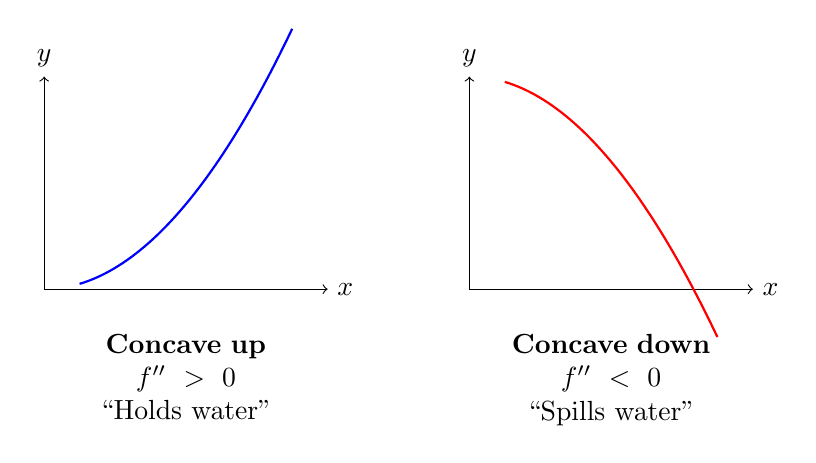
\begin{tikzpicture}[scale=0.9]
    % Concave up
    \begin{scope}[xshift=0cm]
        \draw[->] (0, 0) -- (4, 0) node[right] {$x$};
        \draw[->] (0, 0) -- (0, 3) node[above] {$y$};
        \draw[thick, blue, domain=0.5:3.5, samples=50] plot (\x, {0.3*\x*\x});
        \node[below, text width=3cm, align=center] at (2, -0.5) {
            \textbf{Concave up} \\
            $f'' > 0$ \\
            ``Holds water''
        };
    \end{scope}
    
    % Concave down
    \begin{scope}[xshift=6cm]
        \draw[->] (0, 0) -- (4, 0) node[right] {$x$};
        \draw[->] (0, 0) -- (0, 3) node[above] {$y$};
        \draw[thick, red, domain=0.5:3.5, samples=50] plot (\x, {3 - 0.3*\x*\x});
        \node[below, text width=3cm, align=center] at (2, -0.5) {
            \textbf{Concave down} \\
            $f'' < 0$ \\
            ``Spills water''
        };
    \end{scope}
\end{tikzpicture}
\end{center}

\begin{theorem}[Second Derivative Test]
Let $f''$ be continuous near $c$, and suppose $f'(c) = 0$.
\begin{enumerate}
    \item If $f''(c) > 0$, then $f$ has a local minimum at $c$
    \item If $f''(c) < 0$, then $f$ has a local maximum at $c$
    \item If $f''(c) = 0$, the test is inconclusive
\end{enumerate}
\end{theorem}

\begin{proof}[Proof Sketch]
If $f'(c) = 0$ and $f''(c) > 0$, then $f'$ is increasing near $c$ (since $f' ' > 0$).

Therefore $f' < 0$ for $x < c$ (just left of $c$) and $f' > 0$ for $x > c$ (just right).

So $f$ decreases before $c$ and increases after $c$, making $c$ a local minimum. $\blacksquare$
\end{proof}

\section{L'Hôpital's Rule}

\begin{intuition}
How do we compute limits like $\lim_{x \to 0} \frac{\sin x}{x}$ or $\lim_{x \to \infty} \frac{e^x}{x^2}$?

When both numerator and denominator approach 0 (or both $\infty$), we get indeterminate forms: $\frac{0}{0}$ or $\frac{\infty}{\infty}$.

\textbf{L'Hôpital's Rule}: In such cases, we can differentiate the numerator and denominator separately!
\end{intuition}

\begin{theorem}[L'Hôpital's Rule, 1696]\index{L'Hopital's rule@L'Hôpital's rule}\index{limits!L'Hopital's rule@L'Hôpital's rule}\index{indeterminate forms}
Suppose $f$ and $g$ are differentiable on an open interval $I$ containing $a$ (except possibly at $a$), and $g'(x) \neq 0$ for $x \in I \setminus \{a\}$.

\textbf{Case 1 ($\frac{0}{0}$ form)}: If $\lim_{x \to a} f(x) = 0$ and $\lim_{x \to a} g(x) = 0$, and if $\lim_{x \to a} \frac{f'(x)}{g'(x)}$ exists, then:
\[\lim_{x \to a} \frac{f(x)}{g(x)} = \lim_{x \to a} \frac{f'(x)}{g'(x)}\]

\textbf{Case 2 ($\frac{\infty}{\infty}$ form)}: If $\lim_{x \to a} |g(x)| = \infty$ and $\lim_{x \to a} \frac{f'(x)}{g'(x)}$ exists, then:
\[\lim_{x \to a} \frac{f(x)}{g(x)} = \lim_{x \to a} \frac{f'(x)}{g'(x)}\]

The theorem also holds for one-sided limits and limits at $\pm\infty$.
\end{theorem}

\begin{proof}[Proof of Case 1 (Sketch)]
We prove the $\frac{0}{0}$ case. Assume $f(a) = g(a) = 0$ (extend by continuity if needed).

For $x$ near $a$ (but $x \neq a$), apply the Cauchy Mean Value Theorem (a generalization of MVT):

There exists $c$ between $a$ and $x$ such that:
\[\frac{f(x) - f(a)}{g(x) - g(a)} = \frac{f'(c)}{g'(c)}\]

Since $f(a) = g(a) = 0$:
\[\frac{f(x)}{g(x)} = \frac{f'(c)}{g'(c)}\]

As $x \to a$, we have $c \to a$ (since $c$ is between $a$ and $x$).

If $\lim_{x \to a} \frac{f'(x)}{g'(x)} = L$, then:
\[\lim_{x \to a} \frac{f(x)}{g(x)} = \lim_{c \to a} \frac{f'(c)}{g'(c)} = L\]
$\blacksquare$
\end{proof}

\begin{warning}
\textbf{Common mistakes}:

\begin{enumerate}
    \item L'Hôpital's Rule is \textbf{NOT} the Quotient Rule!
    
    We differentiate numerator and denominator \textit{separately}, not as a quotient:
    \[\lim_{x \to a} \frac{f(x)}{g(x)} = \lim_{x \to a} \frac{f'(x)}{g'(x)} \quad \text{(L'Hôpital)}\]
    NOT:
    \[\lim_{x \to a} \frac{f(x)}{g(x)} = \lim_{x \to a} \frac{f'(x)g(x) - f(x)g'(x)}{g(x)^2} \quad \text{(Quotient Rule)}\]
    
    \item Only use L'Hôpital when you have indeterminate form $\frac{0}{0}$ or $\frac{\infty}{\infty}$
    
    \item If $\lim_{x \to a} \frac{f'(x)}{g'(x)}$ doesn't exist, L'Hôpital's Rule doesn't help (but the original limit might still exist!)
\end{enumerate}
\end{warning}

\begin{example}[Basic Application]
Compute $\lim_{x \to 0} \frac{\sin x}{x}$.

\textbf{Solution}: As $x \to 0$, both $\sin x \to 0$ and $x \to 0$, so we have $\frac{0}{0}$ form.

Apply L'Hôpital's Rule:
\[\lim_{x \to 0} \frac{\sin x}{x} = \lim_{x \to 0} \frac{(\sin x)'}{(x)'} = \lim_{x \to 0} \frac{\cos x}{1} = \cos 0 = 1\]

Therefore $\lim_{x \to 0} \frac{\sin x}{x} = 1$. $\blacksquare$
\end{example}

\begin{example}[Multiple Applications]
Compute $\lim_{x \to 0} \frac{e^x - 1 - x}{x^2}$.

\textbf{Solution}: As $x \to 0$: numerator $\to 0$ and denominator $\to 0$, so $\frac{0}{0}$ form.

Apply L'Hôpital's Rule:
\[\lim_{x \to 0} \frac{e^x - 1 - x}{x^2} = \lim_{x \to 0} \frac{e^x - 1}{2x}\]

Still $\frac{0}{0}$ form! Apply L'Hôpital again:
\[\lim_{x \to 0} \frac{e^x - 1}{2x} = \lim_{x \to 0} \frac{e^x}{2} = \frac{1}{2}\]

Therefore $\lim_{x \to 0} \frac{e^x - 1 - x}{x^2} = \frac{1}{2}$. $\blacksquare$
\end{example}

\begin{example}[$\frac{\infty}{\infty}$ Form]
Compute $\lim_{x \to \infty} \frac{x^2}{e^x}$.

\textbf{Solution}: As $x \to \infty$: both $x^2 \to \infty$ and $e^x \to \infty$, so $\frac{\infty}{\infty}$ form.

Apply L'Hôpital's Rule:
\[\lim_{x \to \infty} \frac{x^2}{e^x} = \lim_{x \to \infty} \frac{2x}{e^x}\]

Still $\frac{\infty}{\infty}$! Apply again:
\[\lim_{x \to \infty} \frac{2x}{e^x} = \lim_{x \to \infty} \frac{2}{e^x} = 0\]

Therefore $\lim_{x \to \infty} \frac{x^2}{e^x} = 0$. 

\textbf{Interpretation}: Exponential functions grow faster than polynomials! $\blacksquare$
\end{example}

\section{Looking Forward: Integration}

\begin{intuition}
Differentiation answers: ``What is the rate of change?''

\textbf{Integration} (next chapter) answers the reverse question: ``What function has this rate of change?''

\textbf{Also}: Integration computes areas, volumes, arc lengths, work, probability distributions, and more.

The \textbf{Fundamental Theorem of Calculus} connects differentiation and integration:
\[\int_a^b f'(x) \, dx = f(b) - f(a)\]

Differentiation and integration are inverse operations---this is the crowning achievement of calculus.
\end{intuition}

\begin{center}
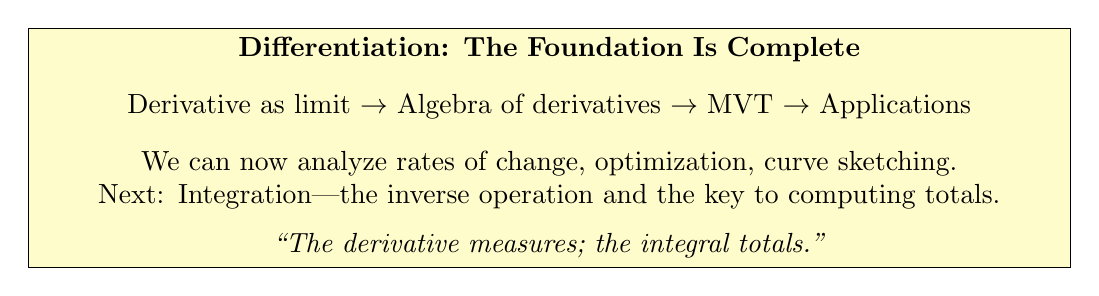
\begin{tikzpicture}[scale=1.0]
    \node[rectangle, draw, fill=yellow!20, text width=13cm, align=center] at (6.5, 0) {
    \textbf{Differentiation: The Foundation Is Complete} \\[0.3cm]
    Derivative as limit $\to$ Algebra of derivatives $\to$ MVT $\to$ Applications \\[0.3cm]
    We can now analyze rates of change, optimization, curve sketching. \\
    Next: Integration---the inverse operation and the key to computing totals. \\[0.2cm]
    \textit{``The derivative measures; the integral totals.''}
    };
\end{tikzpicture}
\end{center}
